% Capítulo 3
\chapter{Arquitetura}
\label{ch:architecture}

\abrv[ARASH -- \textit{Anthropomorphic Robot Augmented with Sense of Human}, em livre tradução Robô Antropomórfico Aumentado com Sentido de Ser Humano]{ARASH}(\textit{Anthropomorphic Robot Augmented with Sense of Human}, em português Robô Antropomórfico Aumentado com Sentido de Ser Humano), além de um herói arqueiro da mitologia iraniana, é um robô de 7,5 Kg e 1 metro de altura. Possuindo 20 graus de liberdade (ou \abrv[DOF -- Do inglês \textit{Degrees Of Freedom}, ou graus de liberdade]{DOF}, do inglês \textit{degrees of freedom}), ele tenta imitar a configuração humana, tanto em suas juntas quanto em suas proporções. Em suas juntas, Arash possui motores MX-28, MX-64 e MX-106 (da Robotis Co), dependendo da carga suportada. Como controlador principal, um computador \textit{mini-box} é utilizado em conjunto com uma placa microcontroladora \textit{OpenCM9.04} que serve de interface entre o controlador principal e os motores.

\section{Visão Geral}
\label{sec:architecture:overview}

Com o passar dos anos, a arquitetura distribuída é vem sendo cada vez mais adotada na robótica. A ideia é que cada componente funcione de forma independente para evitar que uma eventual falha derrube todo o sistema. Componentes individuais podem ser adicionados, ou substituídos, a medida em que melhorias, ou novas capacidades, sejam implementadas.

\begin{figure}[htb]
	\centering
	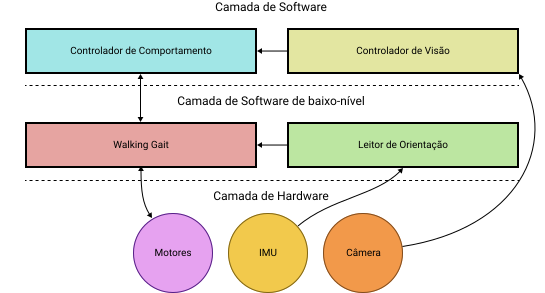
\includegraphics[scale=1]{imagens/svg/softwarearchitecture-flow}
	\caption{Visão simplificada da arquitetura do sistema e seus fluxos.}
	\label{fig:softwarearchitecture:overview}
\end{figure}

Na figura~\ref{fig:softwarearchitecture:overview} é possível observar os principais componentes -- e o sentido do fluxo de dados entre eles -- envolvidos no processo qualquer tarefa básica. Esses componentes são executados em diferentes camadas do sistema. Na arquitetura, existem 3 camadas que podem ser descritas independentemente: A camada de software, a de software de baixo nível, e a de hardware.

Na camada de \textit{hardware}, a mais inferior na figura~\ref{fig:softwarearchitecture:overview}, estão a câmera, a IMU e os motores utilizados nas juntas. Os motores serão melhor descritos na subseção sobre atuadores (subseção~\ref{subsec:Architecture:Atuators}). A IMU, \textit{inertial measurement unit}, que é um sensor eletrônico capaz de medir as forças sofridas por um corpo, é utilizada para ler a orientação do corpo do robô.

A camada de software de baixo nível é responsável pelo processamento de dados da \textit{IMU}, juntamente com a execução do \textit{walking gait}. Esta camada roda dentro da placa microcontroladora \textit{Robotis.Co OpenCM9.04} (com um processador \textit{32bit ARM Cortex-M3}, memória \textit{flash} de 128Kb e 20Kb de \textit{SRAM}), \textit{arduino-like}.

A camada de software é executada dentro do ``controlador principal'', que é um computador \textit{mini-box PC MAXData QutePC-3001} com um processador 64 bits de dois núcleos Intel\copyright{} Celeron\copyright{} 847E (1,1GHz e 2MB de \textit{cache}), rodando o Ubuntu 14.04. Esta camada é responsável por rodar os componentes de software e enviar comandos de controle para a camada inferior de baixo nível.

\subsection{Visão}

Visão não é o foco deste trabalho. Entretanto, uma explanação geral é necessária afim de melhor entender o funcionamento geral do sistema.

\begin{figure}[h!]
	\centering
	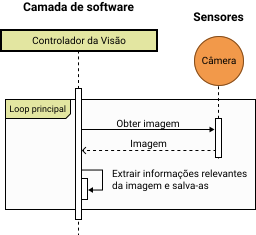
\includegraphics[scale=1]{imagens/svg/softwarearchitecture-vision}
	\caption{Diagrama de sequência do componente de visão.}
	\label{fig:softwarearchitecture:vision}
\end{figure}

O controle de visão é um software que conecta-se via USB com a câmera, analisando as imagens e extraindo informações relevantes à execução da tarefa do robô. De forma geral, podemos abstrair seu funcionamento em duas \textit{threads} distintas:

A primeira é o \textit{loop} principal -- representada na figura \ref{fig:softwarearchitecture:vision} --, onde, sequencialmente, o controlador obtém a imagem da câmera. Em seguida, a extração de informações é realizada. Esse processo depende da tarefa que o robô deve realizar; tais como detectar a bola, os adversários e as linhas do campo, em caso de futebol ou detectar as linhas guia da pista de corrida no caso da maratona. Em seguida, tudo o que foi encontrado é salvo para futuras consultas até que a próxima iteração ocorra e os dados sejam atualizados.

A segunda \textit{thread}, visualizada na figura~\ref{fig:softwarearchitecture:software}, do controle de visão executa o sistema de comunicação que pode ser implementado de várias maneiras, desde objetos \textit{JSON} sendo transmitidos via \textit{UDP} até um \textit{message broker} com filas de consumo. Ao receber a mensagem de solicitação das informações, responde serializando os dados que ficaram salvos na primeira \textit{thread}, fornecendo as informações com atraso mínimo.

\subsection{Controlador de Comportamento}

O controlador de comportamento implementa a tarefa que deve ser realizada pelo robô. Ele funciona como um gerente que coordena outros componentes, recebendo informações e enviando comandos com ações específicas serem a executadas. Na figura~\ref{fig:softwarearchitecture:software} é possível observar a sequência de passos realizados pelo controlador de comportamento.

Usando como exemplo uma partida de futebol, na figura~\ref{fig:softwarearchitecture:software} vemos o controlador de comportamento ``jogador'' consultando o componente de visão, que responde a posição da bola, previamente obtida durante o processo da figura~\ref{fig:softwarearchitecture:vision}. Em seguida, baseado nessas informações o comportamento envia o comando ao \textit{walking gait} para caminhar na direção correta.

\begin{figure}[htb]
	\centering
	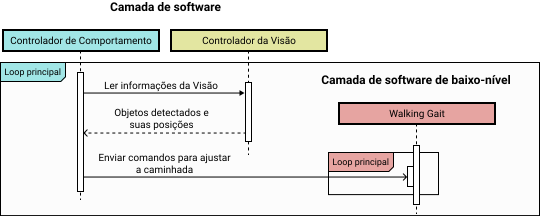
\includegraphics[scale=1]{imagens/svg/softwarearchitecture-software}
	\caption{Diagrama de sequência do controlador de comportamento e suas dependências.}
	\label{fig:softwarearchitecture:software}
\end{figure}

\subsection{\textit{Walking Gait} e Leitor de Orientação}

O componente \textit{walking gait} coordena e executa a caminhada. Ele monitora a USB aguardando os comandos de controle que contém as velocidades da caminhada, enviados a partir do controlador principal.

O componente leitor de orientação desempenha um papel importante dentro do \textit{walking gait}. Ele é o responsável pela verificação da orientação da rotação do torso, uma vez que a \textit{IMU} está situada nas costas de Arash. Desta forma, o \textit{walking gait} faz correções nas juntas para compensar um eventual desvio na trajetória.

\begin{figure}[htb]
	\centering
	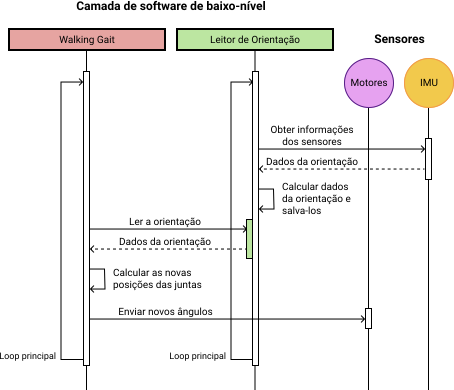
\includegraphics[scale=0.8]{imagens/svg/softwarearchitecture-lowlevel}
	\caption{Diagrama de sequência do \textit{walking gait} e do leitor de orientação.}
	\label{fig:softwarearchitecture:lowlevel}
\end{figure}

Dentro da placa microcontroladora \textit{OpenCM9.04}, o \textit{walking gait} e o leitor de orientação rodam em \textit{threads} dinstintas, recurso este habilitado pela biblioteca \textit{MapleFreeRTOS}. Na figura~\ref{fig:softwarearchitecture:lowlevel} observa-se a execução de ambas a \textit{threads} separadamente e a forma de interação entre elas.	

No componente leitor de orientação, os dados são coletados da \textit{IMU} e um processo de utilizando filtro de \todo{Explicar este processo melhor}\textit{Kalman} é utilizado para obter ua estimativa mais acurada das orientações que são salvas em variáveis. Já na \textit{thread} que roda o \textit{walking gait}, a orientação é continuamente consultada e utilizada para que os ângulos das juntas sejam atualizados.

\subsection{Graus de Liberdade e Atuadores}
\label{subsec:architecture:Atuators}

\todo{Adicionar um parágrafo introdutório.}
PARAGRAFO INTRODUTÓRIO.

Tão importante quanto a configuração das juntas é a orientação dos atuadores para que os cálculos funcionem como o esperado.

\begin{figure}[htb]
	\centering
	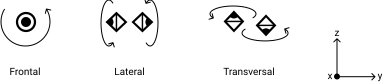
\includegraphics[scale=1]{imagens/svg/actuators-orientation}
	\caption{Orientação dos movimentos dos atuadores}
	\label{fig:ActuatorsOrientation}
\end{figure}

A figura~\ref{fig:ActuatorsOrientation} exibe as possíveis orientações dos atuadores que são referenciadas ao longo do trabalho como frontal, lateral e transversal.

Atuadores com orientação frontal -- ou simplesmente, atuadores frontais -- propiciam rotação orientada pelo eixo $X$, que está aponta para o leitor (para fora do papel). Esse tipo de rotação também é referida como \textit{roll}.

Atuadores laterais apontam para direita ou esquerda. Eles apresentam rotação com base no eixo $Y$ (plano $XZ$), também conhecida como rotação \textit{pitch}. Analogamente, atuadores transversais apontam para cima ou baixo, com base no eixo $Z$ (plano $XY$), com movimento de rotação conhecido como \textit{yaw}.

Na figura~\ref{fig:architecture:arash:actuators_orientations}, observa-se o esquema de orientação dos atuadores aplicada no diagrama das juntas de Arash. Ainda na mesma figura, os ``triângulos pretos preenchidos'' representam apenas o fim de uma cadeia de atuadores. Assim, estes símbolos representam as mãos, que não possuem atuadores, e a ponta da cabeça, onde encontra-se a câmera. 

Estas orientações são importantes durante os cálculos dos ângulos enviados às juntas. Já que a inconsistência do modelo matemático e o robô físico causa inversão de movimentos durante a caminhada, causando reações inesperadas e possíveis danos.

Em Arash, todos os atuadores utilizados são produzidos pela Robotics.Co. Porém, devido a variação de carga nas diversas juntas, foram utilizados diferentes  modelos da série MX. Esta decisão de projeto diminui bastante o custo final do robô.

\begin{figure}[htb]
	\centering
	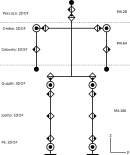
\includegraphics[scale=1]{imagens/svg/arash-schematics}
	\caption{Diagrama de orientação dos atuadores de Arash}
	\label{fig:architecture:arash:actuators_orientations}
\end{figure}

No pescoço, onde a carga é bem leve, ``MX-28'' são suficientes. Dois atuadores, um na posição transversal (o atuador mais baixo) que fornece o movimento panorâmico a cabeça e outro na posição horizontal, fornecendo o movimento de inclinação vertical da cabeça.

Nos braços, que podem sofrer uma carga maior, atuadores ``MX-64'' são utilizados. Isso é importante já que existem modalidades de competições, como o levantamento de peso, que testam a capacidade do carregamento de cargas.

Para as pernas, foram utilizados atuadores ``MX-106'' que são mais poderosos que os anteriores. Entretanto, na fase de projeto, simulações mostraram que durante o movimento de levantar-se do chão (em caso da recuperação de uma possível queda), o torque nas juntas do joelho era levado ao máximo suportado pelo ``MX-106'', podendo assim levar este motor à falha. Desta forma, 2 atuadores sincronizados passaram a formar esta junta, afim de compartilhar a carga sofrida entre dois motores. Esta junta dupla não oferece nenhum impacto na implementação, já que os motores da série ``MX-106'' oferecem a capacidade de serem ligados e sincronizados via \textit{hardware}. Assim, a nível de software controla-se apenas 1 único atuador. Desta forma, apesar das 20 DOF, Arash possui 22 motores.

\section{A nova arquitetura}

De acordo com os problemas e solução já discutidos em seções anteriores, esta seção irá apresentar as mudanças realizadas na arquitetura original apresentada na seção~\ref{sec:architecture:overview}.

\begin{figure}[h!]
	\centering
	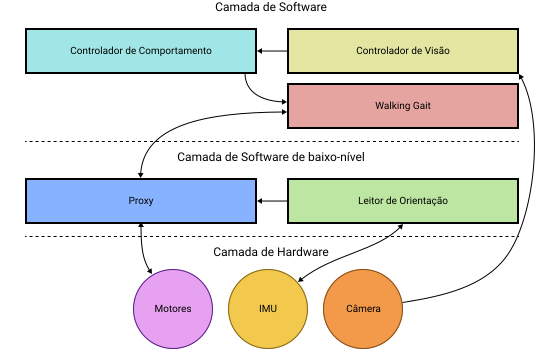
\includegraphics[scale=1]{imagens/svg/softwarearchitecture-newproposal}
	\caption{Diagrama de orientação dos atuadores de Arash.}
	\label{fig:softwarearchitecture:newproposal}
\end{figure}

A figura~\ref{fig:softwarearchitecture:newproposal} mostra o \textit{walking gait} -- agora na camada de software -- funcionando dentro do controlador principal, e um novo compontente chamado \textit{proxy} é apresentado como interface os componentes de hardware e o \textit{walking gait}. O papel do novo componente é de servir realmente como um \textit{proxy} enviando comandos recebidos do controlador principal aos motores e também receber a orientação do componente leitor de orientação e fornecê-la ao controlador principal.

O controlador de comportamento continua a enviar os comandos de controle ao \textit{walking gait}. Porém, ao invés de usar \todo{Especificar esses comandos na seção onde fala sobre esses comandos}comandos binários via USB, agora utiliza objetos serializados via \textit{JSON} \todo{Justificar por que via rede}via rede. 

Entre o \textit{walking gait} e o \textit{proxy} a comunicação ocorre via USB @ 1 Mbps. Comandos de controle utilizando o \textit{dynamixel protocol 1.0} são gerados e enviados diretamente do \textit{walking gait} ao \textit{proxy}, que apenas os encaminha aos motores. Esta estratégia foi adotada para habilitar a possibilidade da utilização de motores de diferentes tipos, não apenas da Robotis Co. Assim, apenas o \textit{walking gait} é responsável pela geração de destes comandos específicos de cada motor enquanto o \textit{proxy} apenas os encaminha.

Na camada de software de baixo nível, o leitor de orientação fornece os dados de orientação ao \textit{proxy} que encarrega-se de disponibiliza-los ao \textit{walking gait}.

\begin{figure}[h!]
	\centering
	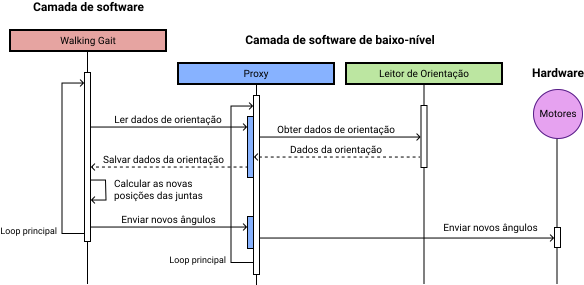
\includegraphics[scale=1]{imagens/svg/softwarearchitecture-newproposal-sequence}
	\caption{Diagrama de sequência simplificado com as modificações na arquitetura.}
	\label{fig:softwarearchitecture:newproposal:sequence}
\end{figure}

Na figura~\ref{fig:softwarearchitecture:newproposal:sequence}, é possível observar o diagrama de sequência com os componentes que foram atingidos pela mudança na arquitetura.

Nessa nova versão da arquitetura os cálculos dos ângulos das juntas são realizados pela nova implementação do \textit{walking gait}. Para tanto, ele precisa dos dados de orientação que devem ser fornecidos pelo componente leitor de orientação, que ainda encontra-se dentro da \textit{OpenCM9.04}. Após os cálculos realizados agora o \textit{walking gait} deve comunicar-se com o \textit{proxy} que encaminhará os novos ângulos aos motores.

\section{\textit{Walking gait}}

Nesta seção detalhes arquiteturais da implementação do \textit{walking gait} serão descritos.

O \textit{walking gait} é o componente que coordena a caminhada mantendo o estado drobô, sabendo onde cada perna encontra-se e o seu estágio durante a caminhada. Desta forma, quando algum evento de perturbação, ou de ajuste, é disparado o \textit{walking gait} inicia a atualização das juntas a partir do estado atual. Assim, podemos descrever a caminhada como um evento contínuo no tempo.

Para realizar a tarefa de forma adequada, o componente faz uso de multi-processamento. Três \textit{threads} dentro do componente são responsáveis por tarefas específicas essenciais ao complemento do comportamento geral da caminhada: A \textit{thread} de rede, a \textit{thread} atualização dos motores e a \textit{thread} principal.

\subsection{\textit{Thread} principal: Da geração da trajetória até a aplicação às juntas}

\begin{figure}[h!]
	\centering
	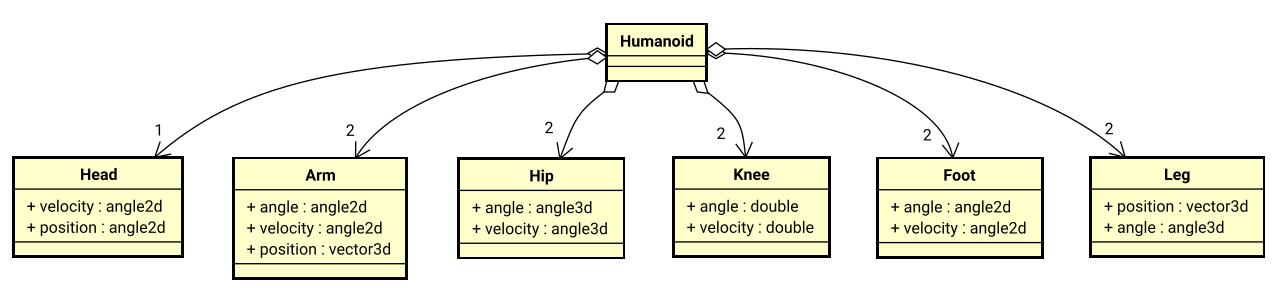
\includegraphics[scale=0.4]{imagens/svg/walkinggait-domain}
	\caption{Diagrama de domínio do \textit{walking gait}.}
	\label{fig:walkinggait:domain}
\end{figure}

A figura~\ref{fig:walkinggait:domain} mostra o diagrama de domínio das classes relevantes aos dados que o componente manipula. Nela podemos ver a classe $Humanoid$ é uma agregação de diversas outras classes que representam cada parte de Arash. É possível também observar que nas classes $Head$, $Arm$, $Hip$, $Knee$, $Foot$ existem dados ângulo e velocidade. Isso se dá por causa que componente utiliza essas informações para calcular o próximo estado do sistema em caso de algum distúrbio. Nota-se também, que a classe $Leg$ aparece de forma ambígua, já que existem as definições de $Hip$, $Knee$ e $Foot$. Porém, a classe $Leg$, representa os dados da cinemática inversa de uma perna, enquanto as demais classes guardam o estado atual das partes que representam.

Nota-se, também, a notação dos dados utilizados: $angle2d$, $angle3d$ e $vector3d$. Note que todos os tipos possuem o sufixo numérico, que indica a quantidade de dimensões aquela classe guarda, e a letra, que indica o tipo de seus dados, no caso $d$ que significa $double$. Para ângulos, $2$ dimensões significa que as dimensões $pitch$ e $roll$ são guardadas; já para $3$ dimensões as orientações $roll$, $pitch$ e $yaw$ são guardadas. Para vetores, os valores $x$, $y$ e $z$ são guardados.

\subsection{Servidor de controle}

A \textit{thread} de rede roda um servidor \textit{UDP} que aceita objetos serializandos em \textit{JSON} contendo informações de controle.

\subsection{Abstração dos motores}
\label{subsec:motors_abstraction}